\documentclass{article}

\usepackage{graphicx}
\usepackage{tikz}
\usepackage{tikzsymbols}
\usetikzlibrary{calc,patterns,shapes.geometric}
\pagestyle{empty}
\usepackage[margin=0pt]{geometry}
\geometry{papersize={14in,12in}}

\def\centerarc[#1](#2)(#3:#4:#5){\draw[#1] ($(#2)+({#5*cos(#3)},{#5*sin(#3)})$) arc (#3:#4:#5);}

\begin{document}
	\begin{figure}
		\centering
		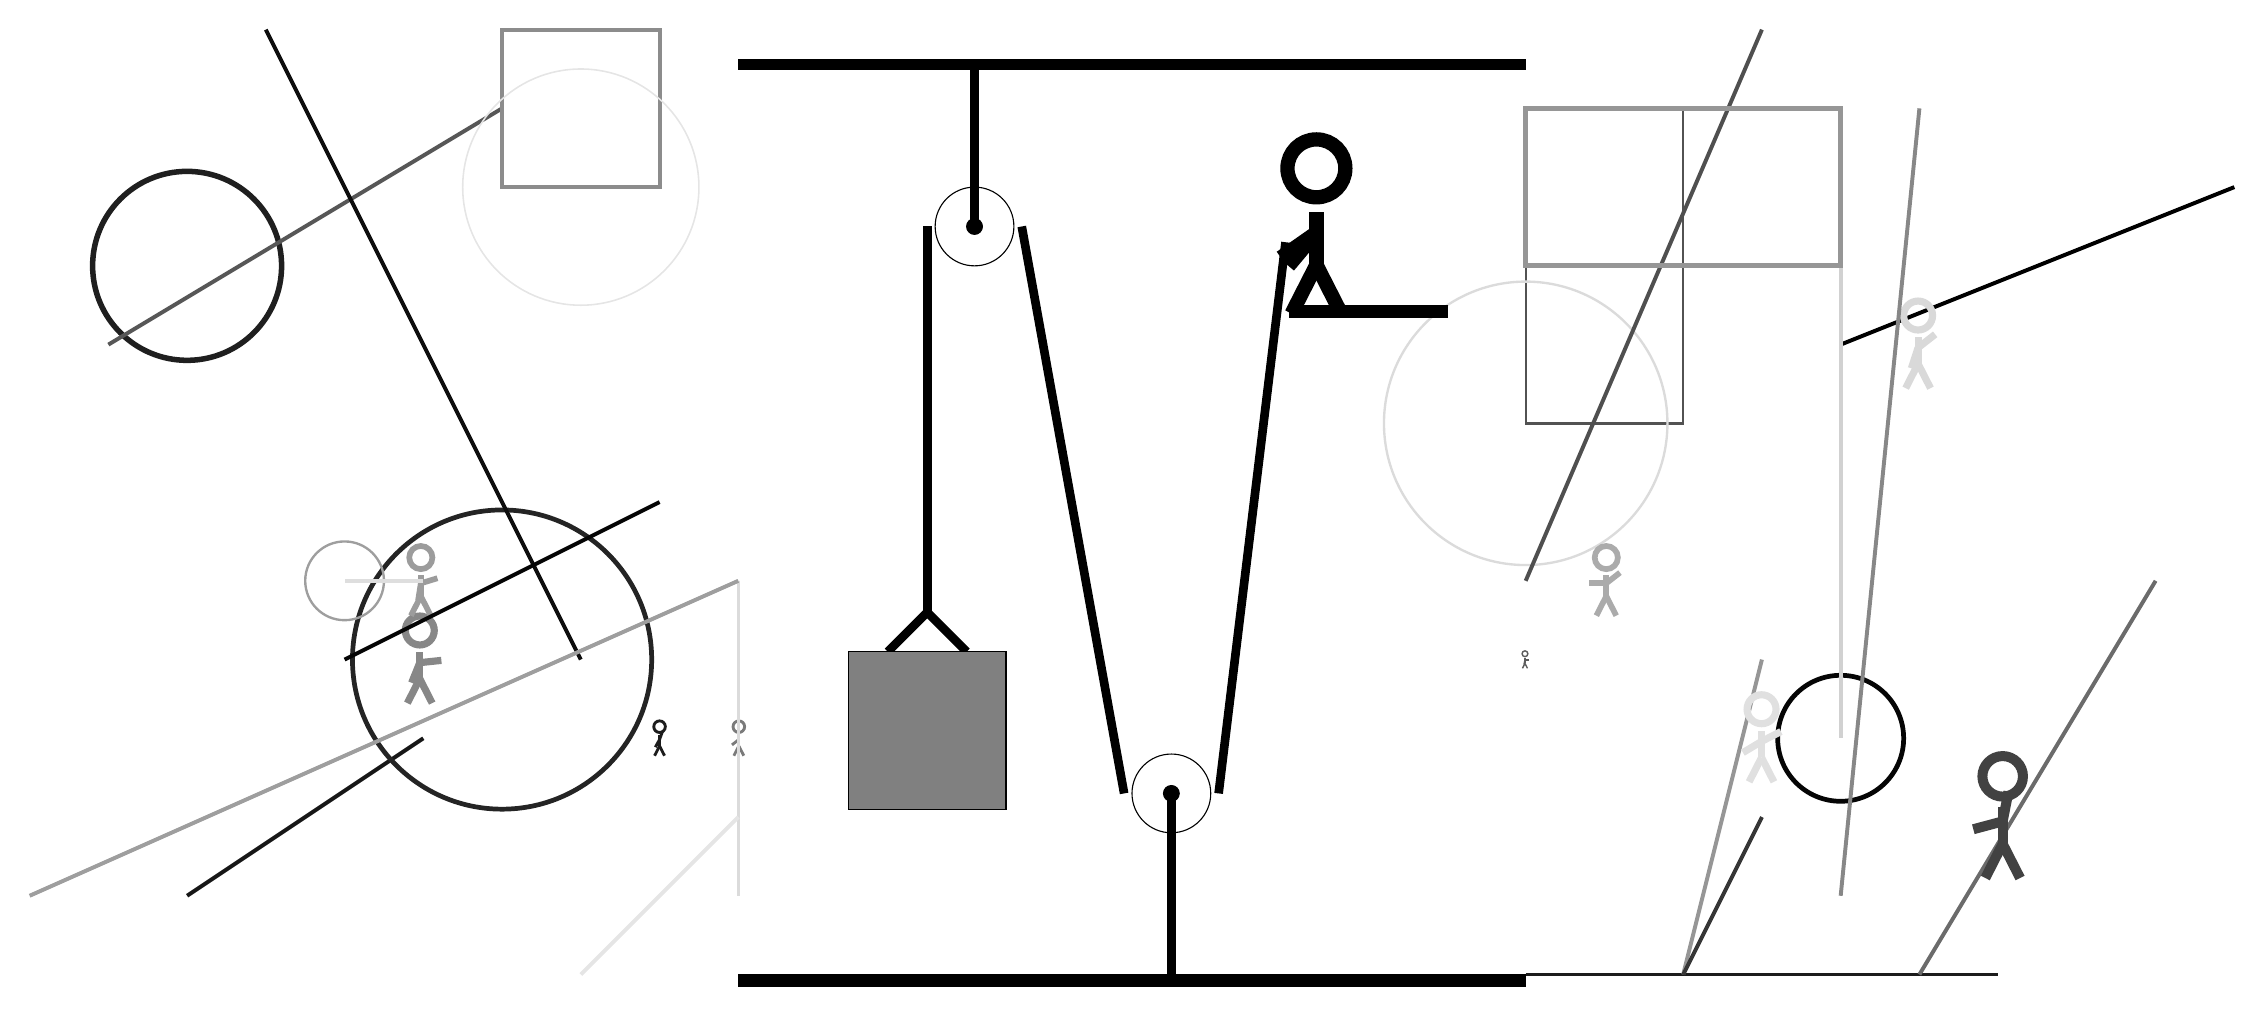
\begin{tikzpicture}
			%%%%% START %%%%%
			
			\draw[fill=black] (-2, 11.5) rectangle (8, 11.625);
			
			\node[line width=0.2mm, color=black!52] at (-2, 3) {\Strichmaxerl[2][38][90]};
			
			\draw[line width=0.3mm, color=black!68] (8, 11) rectangle (10, 7);
			\draw[line width=0.5mm, color=black!89](8, 0) -- (14, 0);
			\draw[line width=0.5mm, color=black!100](12, 8) -- (17, 10);
			
			\draw [line width=0.3mm, color=black!14](8, 7) circle (1.8);
			\node[line width=0.2mm, color=black!47] at (-6, 4) {\Strichmaxerl[5][68][6]};
			
			\draw [line width=0.6mm, color=black!98](12, 3) circle (0.8);
			\draw[line width=0.5mm, color=black!69](8, 5) -- (11, 12);
			\node[line width=0.2mm, color=black!15] at (13, 8) {\Strichmaxerl[5][72][38]};
			
			\node[line width=0.2mm, color=black!33] at (9, 5) {\Strichmaxerl[4][0][38]};
			
			\node[line width=0.3mm, color=black!39] at (-6, 5) {\Strichmaxerl[4][81][17]};
			
			\draw [line width=0.7mm, color=black!88](-9, 9) circle (1.2);
			\draw[line width=0.4mm, color=black!14] (-2, 1) rectangle (-2, 5);
			
			\draw[line width=0.5mm, color=black!91](-6, 3) -- (-9, 1);
			\draw[line width=0.5mm, color=black!66](-5, 11) -- (-10, 8);
			\draw[line width=0.5mm, color=black!47](12, 1) -- (13, 11);
			
			\draw[line width=0.5mm, color=black!18](12, 10) -- (12, 3);
			
			\draw[line width=0.5mm, color=black!41](10, 0) -- (11, 4);
			\draw[line width=0.5mm, color=black!45] (-3, 10) rectangle (-5, 12);
			\draw [line width=0.6mm, color=black!86](-5, 4) circle (1.9);
			\draw[line width=0.5mm, color=black!95](-4, 4) -- (-8, 12);
			
			\draw [line width=0.2mm, color=black!10](-4, 10) circle (1.5);
			
			\draw [line width=0.3mm, color=black!38](-7, 5) circle (0.5);
			\draw[line width=0.6mm, color=black!41] (8, 11) rectangle (12, 9);
			\draw[line width=0.5mm, color=black!58](13, 0) -- (16, 5);
			
			\node[line width=0.4mm, color=black!89] at (-3, 3) {\Strichmaxerl[2][61][70]};
			\draw[line width=0.5mm, color=black!98](-7, 4) -- (-3, 6);
			\node[line width=0.2mm, color=black!12] at (11, 3) {\Strichmaxerl[5][31][27]};
			\draw[line width=0.5mm, color=black!13](-6, 5) -- (-7, 5);
			\draw[line width=0.5mm, color=black!79](10, 0) -- (11, 2);
			\node[line width=0.4mm, color=black!64] at (8, 4) {\Strichmaxerl[1][77][0]};
			
			\draw[line width=0.5mm, color=black!10](-2, 2) -- (-4, 0);
			\node[line width=0.4mm, color=black!74] at (14, 2) {\Strichmaxerl[7][15][79]};
			
			\draw[line width=0.5mm, color=black!38](-2, 5) -- (-11, 1);
			
			\draw (3.5, 2.3) circle (0.5);
			\draw[fill=black] (3.5, 2.3) circle (0.1);
			\draw[line width=1.1mm] (3.5, 2.3) -- (3.5, 0);
			
			\draw (1, 9.5) circle (0.5);
			\draw[fill=black] (1, 9.5) circle (0.1);
			\draw[line width=1.1mm] (1, 11.5) -- (1, 9.5);
			
			\draw[line width=1.1mm](-0.1, 4.1) --  (0.4, 4.6) -- (0.9, 4.1);
			\draw[fill=black!50] (-0.6, 4.1) rectangle (1.4, 2.1);
			
			\draw[line width=1.1mm](0.4, 9.5) -- (0.4, 4.6);
			\centerarc[line width=1.1mm](1, 9.5)(180:0:0.6)
			\draw[line width=1.1mm](1.6, 9.5) -- (2.9, 2.3);
			\centerarc[line width=1.1mm](3.5, 2.3)(180:360:0.6)
			\draw[line width=1.1mm](4.1, 2.3) -- (4.95, 9.3);
			
			\node at (5.3, 9.5) {\Strichmaxerl[10][35][-130]};
			\draw[fill=black] (5, 8.5) rectangle (7, 8.35);
			
			\draw[fill=black] (-2, 0) rectangle (8, -0.15);
			
			%%%%% END %%%%%
		\end{tikzpicture}
	\end{figure}	
\end{document}